\documentclass[12pt,a4paper]{beamer}
\usetheme{Amsterdam}
%\usecolortheme{beaver}
\usepackage[english,french]{babel}
%\usepackage[utf8]{inputenc}  
\usepackage[T1]{fontenc}
\usepackage{fontspec}
\usepackage{amsmath}
\usepackage{amsfonts}
\usepackage{amssymb}
\usepackage{tikz}
\usepackage{listings}
\usepackage{pgfplots}
%\pgfplotsset{compat=1.14}
\pgfplotsset{compat=newest}
\usepackage{color}
\usepackage{marvosym}

%Underline in color
\newcommand{\coloruline}[3]{\emph{\textcolor{#1}{\underline{#2\textcolor{black}{#3}}}}}



\lstset{
  language=Java,
  commentstyle=\color{mygreen},    % comment style
  stringstyle=\color{mymauve},     % string literal style
  keywordstyle=\color{blue},       % keyword style
  basicstyle=\footnotesize        % the size of the fonts that are used for the code
}

\title{\textbf{Algorithmique avancée}}
\subtitle{Arbres binaires de recherche}
\author{Frédéric Guyomarch}
\date{2018/2019 - Semestre 3}
\institute % (optional)
{

  Université de Lille1\\
  IUT-A de Lille

}
 

 
\logo{
\includegraphics[width=5em]{figs/iutaustl}}

%Remove Figure prefix on captures
\setbeamertemplate{caption}{\raggedright\insertcaption\par}

%Remove Control bar
\beamertemplatenavigationsymbolsempty

\setbeamertemplate{blocks}[rounded]
\newcommand{\hl}[1]{\textcolor{blueemph}{#1}}


\definecolor{mygreen}{rgb}{0,0.6,0}
\definecolor{mygray}{rgb}{0.5,0.5,0.5}
\definecolor{mymauve}{rgb}{0.58,0,0.82}
\definecolor{greenfluo}{rgb}{0,255,0}
\definecolor{blueemph}{RGB}{17,59,94}


\begin{document}

\begin{frame}
\titlepage
\end{frame}


\begin{frame}{Introduction}{Les arbres}

On a vu des structures de base linéaires : 
\begin{itemize}
\item Des tableaux
\item Des listes chaînées
\end{itemize}
Les arbres permettent de \emph{hiérarchiser} l'information.
\begin{block}{Définition}
Un arbre est un graphe non orienté, acyclique et connexe.
\end{block}
\end{frame}

\begin{frame}{Les arbres}{Exemple}
\begin{itemize}
\item Organigramme
\item Système de fichiers
\item Expressions arithmétiques
\item Tableau d'élimination direct en sport
\end{itemize}

\end{frame}



\begin{frame}{Terminologie}{}

\begin{itemize}
\item La terminologie est empruntée aux arbres 
\begin{itemize}
\item généalogiques : père, fils, descendant...
\item naturels : feuille, branche, racine...
\end{itemize} 
\end{itemize}
Un arbre est composé de \hl{n\oe uds} reliés entre eux par des \hl{arêtes}.
\begin{itemize}
\item La \hl{racine} est l'unique n\oe ud au sommet de l'arbre. 
\item Chaque n\oe ud (hormis la racine) est le \hl{fils} de son prédécesseur dans l'arbre qui est son \hl{père}. 
\item Les n\oe uds qui n'ont pas de fils sont des \hl{feuilles}.
\end{itemize}
\end{frame}

\begin{frame}{Terminologie}{}

\begin{itemize}
\item On dit qu'il y a un \hl{chemin} entre deux n\oe uds si il est possible d’accéder de l'un à l'autre en passant par les arrêtes.
\item Le \hl{niveau} d'un n\oe ud est le nombre de génération(s) qui le sépare de la racine.
\item La \hl{hauteur} est le nombre maximum de niveaux.
\item Le \hl{degré} ou l'\hl{arité} d'un n\oe ud est le nombre de ses fils.
\item Un arbre d'arité $n$ est un arbre dont le degré maximum de ses n\oe uds est $n$.
\end{itemize}

\end{frame}

\begin{frame}{Terminologie}{}
\begin{figure}
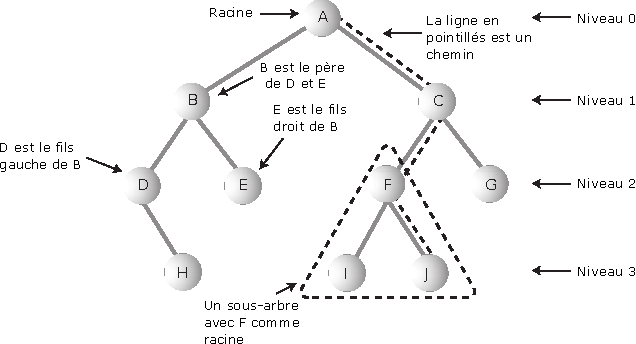
\includegraphics[scale=1]{figs/tree}
\end{figure}
H, E, I, J et G sont des feuilles.

\end{frame}

\begin{frame}{Récursivité}
L'arbre est une structure récursive qui peut être vue : 
\begin{itemize}
\item Soit comme vide
\item Soit comme un arbre dont les fils sont des sous-arbres. 
\end{itemize}
\begin{figure}
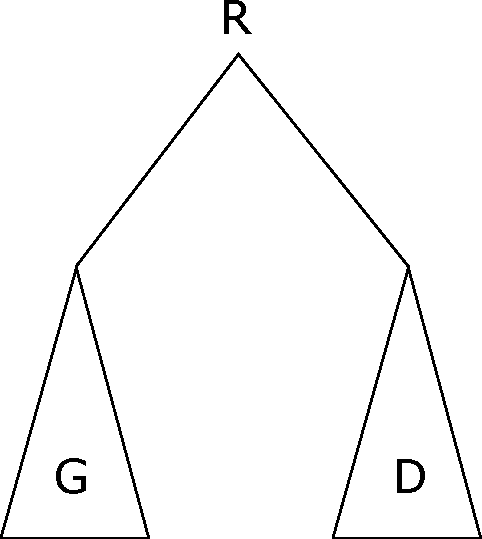
\includegraphics[scale=0.4]{figs/rec_tree}
\end{figure}

\end{frame}


\begin{frame}{Arbre binaire}
\begin{block}{Définitions}
Un arbre d'arité 2 est un \hl{arbre binaire}. Il a au maximum deux fils, un fils gauche et un fils droit.\\
Un arbre binaire est dit \hl{pur} si chacun des n\oe uds a soit exactement 2 fils, soit aucun.
\end{block}

%Un \hl{arbre binaire de recherche} (ABR) est un type de données abstrait constitué d'un couple (clé,valeur).
\end{frame}


\begin{frame}{ABR}
Un \hl{arbre binaire de recherche} (ABR) est un type de données abstrait.
\begin{itemize}
\item Chaque élément a une clé unique, i.e une clé identifie un
élément de façon unique.
\item Les clés dans un sous arbre gauche non vide doivent être
inférieures à la clé de la racine de ce sous arbre.
\item Les clés dans un sous arbre droit non vide doivent être
supérieures à la clé de la racine de ce sous arbre.
\item Les sous arbres gauche et droit sont aussi des arbres
binaires de recherche. (structure récursive).
\end{itemize}

\end{frame}

\begin{frame}{ABR}{Exemple}
\begin{figure}
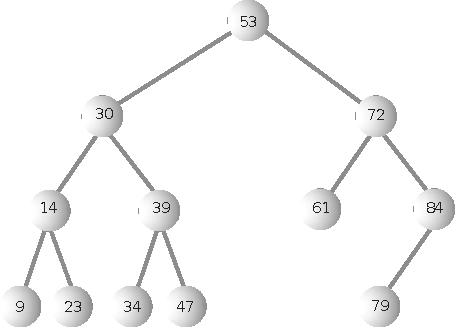
\includegraphics[scale=1]{figs/abr}
\caption{Un arbre binaire de recherche}
\end{figure}

\end{frame}

\begin{frame}{ABR}
On peut définir les opérations suivantes pour un ABR :
\begin{itemize}
\item \texttt{estVide()} : retourne vrai si l'arbre $A$ est vide
\item \texttt{estFeuille(K cle)} : retourne vrai si l'élément de clé $cle$ est une feuille\item \texttt{estRacine(K cle)} : retourne vrai si l'élément de clé $cle$ est la racine
\item \texttt{recherche(K cle)} : retourne l'élément de clé $cle$
\item \texttt{insertion(K cle, V val)} : insertion d'un élément de clé $cle$ et de valeur $val$.
\item \texttt{suppression(K cle)} : suppression d'un élément de clé $cle$.

\end{itemize}
\end{frame}

\begin{frame}{ABR}{Comparaisons}
Quid de l'efficacité d'un ABR par rapport aux tables de hachage, aux tableaux ordonnés ou encore aux listes?
\end{frame}


\begin{frame}{ABR}{Propriétés}
\begin{itemize}
\item Nombre maximal de n\oe uds :
\begin{itemize}
\item Le nombre maximal de n\oe uds de niveau $i$ dans un arbre
binaire est $2^{i-1} , i >= 1$
\item Le nombre maximal de n\oe uds dans un arbre binaire de
profondeur $k$ est $2^{k}-1, k >= 1$
\item Arbre binaire \hl{complet} de profondeur k est un arbre
binaire ayant $2^{k}-1$ n\oe uds.
\begin{itemize}
\item Tous les n\oe uds possèdent 0 ou 2 fils.
\item Le nombre maximal de n\oe uds est atteint donc toutes les feuilles sont au niveau k
\end{itemize}
\end{itemize}
\end{itemize}
\textbf{Question} : Dans un ABR complet de 20 n\oe uds, où l'on considère que la racine est au niveau 1, combien il y a de n\oe uds au niveau 5?
\end{frame}

\begin{frame}{Représentation d'un arbre}{Par chaînage}
A la manière des listes, on peut utiliser une représentation chaînée.
\begin{figure}
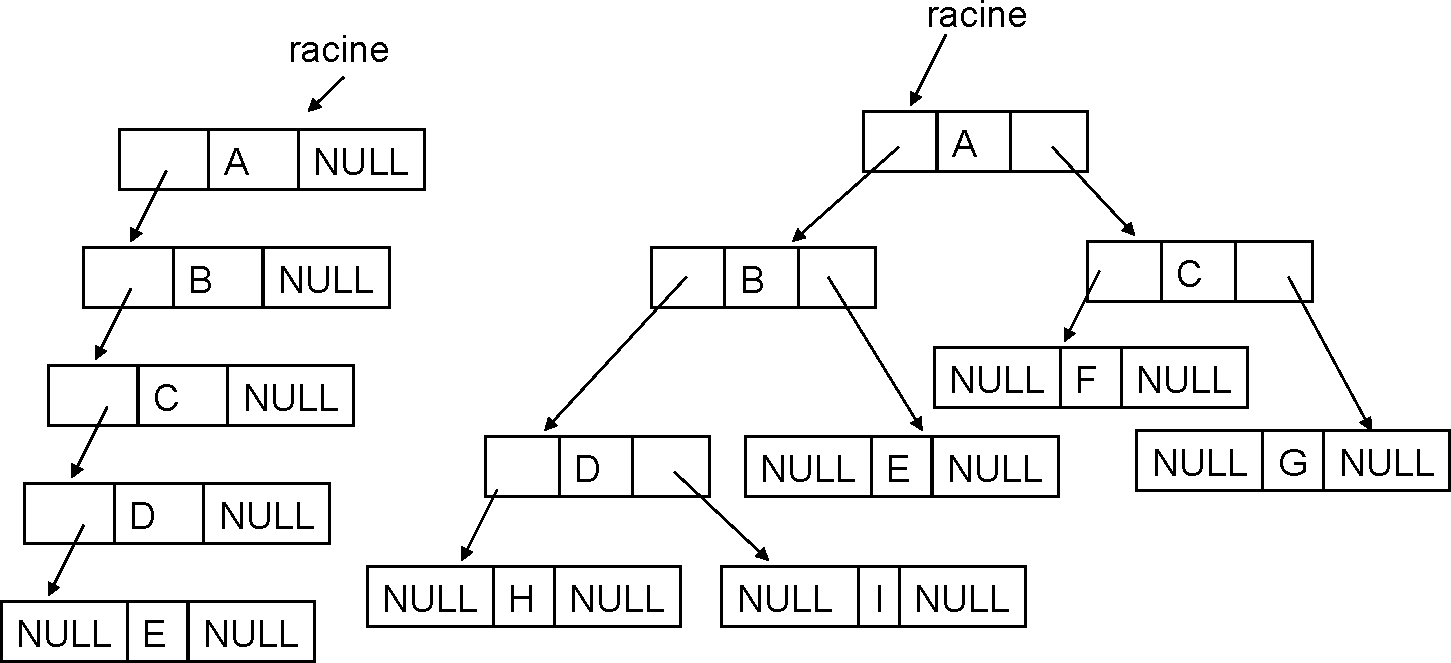
\includegraphics[scale=0.4]{figs/tree_chainage}
\end{figure}


\end{frame}

\begin{frame}{Représentation}{Par tableau}
Il existe également une représentation par tableau:
\begin{figure}
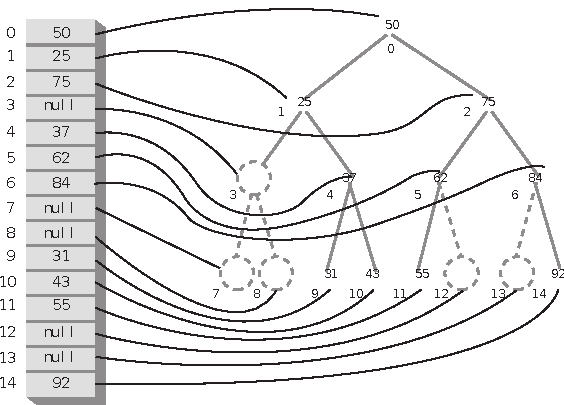
\includegraphics[scale=0.8]{figs/array_tree}
\end{figure}
\end{frame}

\begin{frame}{Représentation}{Par tableau}
\begin{itemize}
\item Gaspillage probable de mémoire
%\item Insertions et suppressions coûteuses
\item Si un n\oe ud a pour indice \texttt{idx}:
\begin{itemize}
\item Son fils droit a pour indice $2 * idx + 2$
\item Son fils gauche a pour indice $2 * idx + 1$
\item Son père a pour indice $(idx-1)/2$
\end{itemize}
\end{itemize}
Nous préférerons le plus souvent la représentation chaînée.
\end{frame}


\begin{frame}[fragile]{Représentation d'un arbre}{Par chaînage}
\vspace{-2em}
\begin{figure}
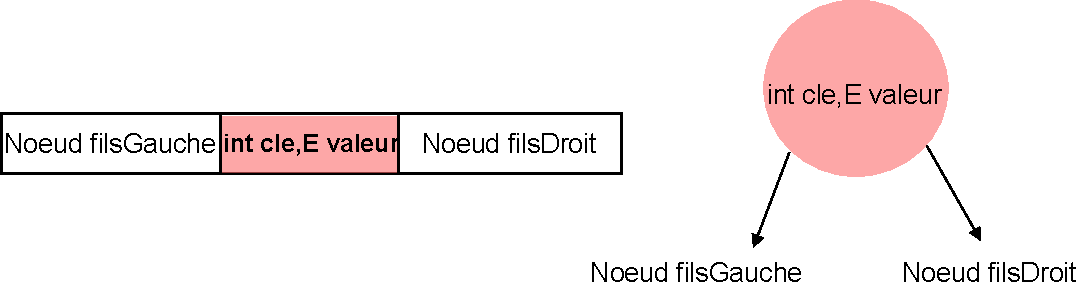
\includegraphics[scale=0.55]{figs/tree_chainage_model}
\end{figure}

\begin{lstlisting}[language=Java]
class Arbre<E>{
  Noeud racine;
}

class Noeud{
  int cle;
  E valeur;
  Noeud filsGauche;
  Noeud filsDroit;
}
\end{lstlisting}

\end{frame}





\begin{frame}{ABR}{Recherche}
\begin{enumerate}
\item Je compare la clé du n\oe ud courant avec la clé recherchée
\item Si elle n'est pas égale alors:
\begin{itemize}
\item Elle est supérieure à la clé recherchée, je regarde le fils gauche
\item Elle est inférieure à la clé recherchée, je regarde le fils droit
\end{itemize}
\item Tant que le n\oe ud courant n'est pas $null$ je réitère les étapes ci-dessus.
\end{enumerate}
\end{frame}

\begin{frame}{ABR}{Recherche}
\begin{figure}
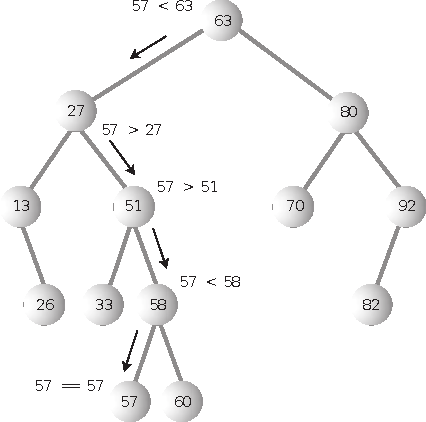
\includegraphics[scale=0.8]{figs/search_abr}
\caption{Recherche de la valeur 57}
\end{figure}
\end{frame}

\begin{frame}[fragile]{ABR}{Recherche itérative}

\begin{lstlisting}[language=Java]
public Noeud recherche(int k){
 Noeud courant = racine;

 while(courant.cle != k){
   if(k < courant.cle)
    courant = courant.filsGauche;
   else
    courant = courant.filsDroit;
   if(courant == null)
    return null;
 }
  return courant;
}

\end{lstlisting}
\end{frame}


\begin{frame}[fragile]{ABR}{Recherche récursive}
\begin{lstlisting}[language=Java]
public Noeud recherche(Noeud noeud, int k){

  if(noeud == null)
   return null;
  
  if(noeud.cle == k)
   return noeud;
  
  if(noeud.cle <= k)
   return recheche(noeud.filsDroit, k);
   
   return recherche(noeud.filsGauche, k);
}
\end{lstlisting}
\end{frame}


\begin{frame}{ABR}{Parcours}

\begin{itemize}
\item On veut visiter une seule fois chacun des n\oe uds de l'arbre
\item On adopte une stratégie de parcours pour parcourir tout l'arbre
\item Soit G,D les parcours des sous-arbres gauche et droit et V la visite le n\oe ud courant (pour obtenir sa valeur par exemple). On peut dégager plusieurs stratégies de parcours, on retiendra:
\begin{itemize}
\item GVD : parcours infixé
\item VGD : parcours préfixé
\item GDV : parcours postfixé
\end{itemize}
\end{itemize}
\hspace{-2em} \textbf{Le sens du parcours va dépendre de l'ordre des appels!
}\end{frame}

\begin{frame}{ABR}{Parcours}
\begin{figure}
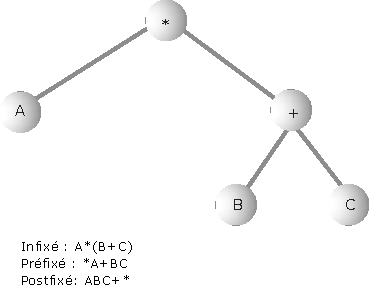
\includegraphics[scale=1]{figs/traversing_tree}
\end{figure}
\end{frame}

\begin{frame}[fragile]{ABR}{Parcours infixe}
\begin{enumerate}
\item Appel récursif sur le fils gauche
\item Visite du n\oe ud courant
\item Appel récursif sur le droit gauche
\end{enumerate}

\begin{lstlisting}[language=Java]
public void parcours(Noeud racine){

  parcours(racine.filsGauche);
  System.out.print(racine.valeur);
  parcours(racine.filsGauche);
  
}
\end{lstlisting}

\end{frame}


\begin{frame}[fragile]{ABR}{Parcours préfixé}
\begin{enumerate}
\item Appel récursif sur le fils gauche
\item Appel récursif sur le droit gauche
\item Visite du n\oe ud courant
\end{enumerate}

\begin{lstlisting}[language=Java]
public void parcours(Noeud racine){

  parcours(racine.filsGauche);
  parcours(racine.filsDroit);
  System.out.print(racine.valeur);

}
\end{lstlisting}

\end{frame}


\begin{frame}[fragile]{ABR}{Parcours postfixé}
\begin{enumerate}
\item Visite du n\oe ud courant
\item Appel récursif sur le fils gauche
\item Appel récursif sur le droit gauche
\end{enumerate}

\begin{lstlisting}[language=Java]
public void parcours(Noeud racine){

  System.out.print(racine.valeur);
  parcours(racine.filsGauche);
  parcours(racine.filsDroit);

}
\end{lstlisting}
\end{frame}

\begin{frame}{ABR}{Parcours}
\begin{figure}
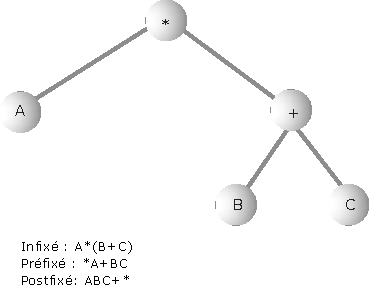
\includegraphics[scale=1]{figs/traversing_tree}
\end{figure}
\end{frame}

\begin{frame}{ABR}{Parcours}
\vspace{-2em}
\begin{figure}
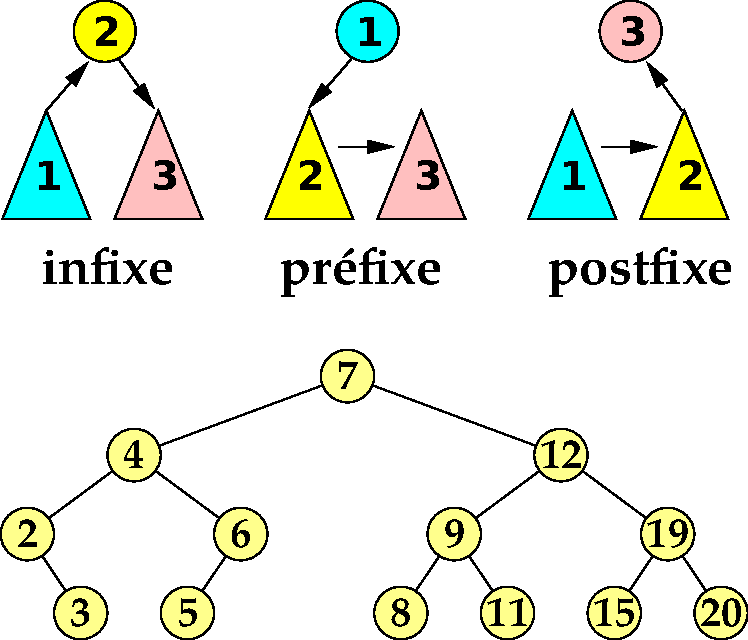
\includegraphics[scale=0.5]{figs/parcours_tree}
\end{figure}
\begin{itemize}
\item Ordre infixe: 2, 3, 4, 5, 6, 7, 8 , 9, 11, 12, 15 ,19, 20. 
\item Ordre préfixe: 7, 4, 2, 3, 6, 5, 12, 9, 8, 11, 19, 15, 20.
\item Ordre postfixe: 3, 2, 5, 6, 4, 8, 11, 9, 15, 20, 19, 12, 7.
\end{itemize}
\end{frame}


\begin{frame}{Parcours}{Efficacité}
\begin{figure}
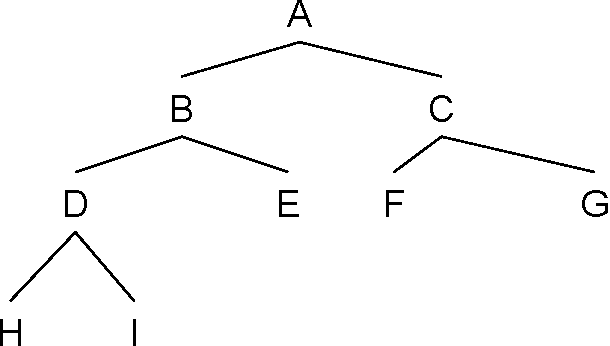
\includegraphics[scale=0.3]{figs/eq_abr}
\caption{Arbre équilibré, nombre de niveaux minimum donc $log(n)$ étapes.}
\end{figure}

\begin{figure}
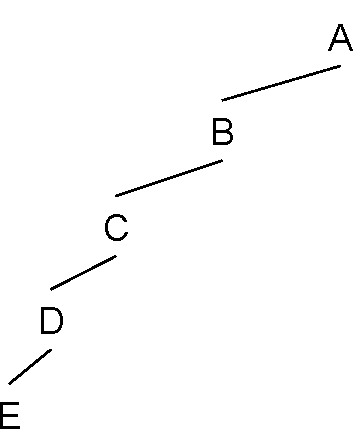
\includegraphics[scale=0.3]{figs/deq_abr}
\caption{Arbre déséquilibré, $n$ étapes.}
\end{figure}
\end{frame}

\begin{frame}{Min/Max}

\begin{figure}
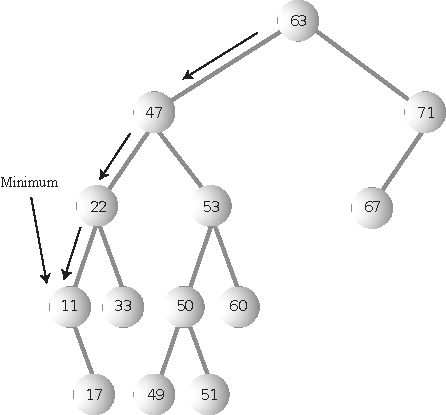
\includegraphics[scale=1]{figs/max_tree}
\end{figure}
\end{frame}

\begin{frame}[fragile]{Min/Max}{Code itératif}
\begin{lstlisting}[language=Java]
public Noeud maximum(){
 Noeud dernier, courant;
 
 courant = racine; 
 
 while(courant!=null){
   dernier = courant;
   courant = courant.fildDroit; 
   //courant = courant.filsGauche pour le min
 }
 return dernier;
}
\end{lstlisting}
\end{frame}


\begin{frame}{Insertion}
\begin{figure}
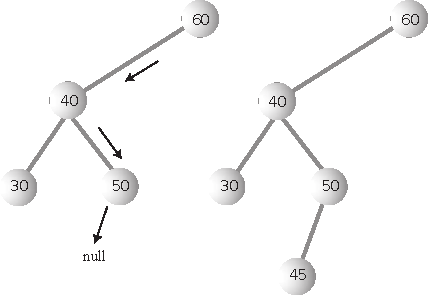
\includegraphics[scale=1]{figs/tree_insertion}
\end{figure}
\hspace{3em}a)Avant insertion  \hspace{1em}  b)Après insertion de 45
\end{frame}

\begin{frame}[fragile]{Insertion}{Version itérative}
\begin{lstlisting}[language=Java]
public void insertion(int cle,E valeur){
  Noeud newNode = new Noeud(cle,valeur);

  if(racine==null) // pas de noeud a la racine
    racine = newNode;
  else{
    Noeud courant = racine; // commence a la racine
    Noeud parent;
    boolean estAjoute = false;
    
\end{lstlisting}
\end{frame}

\begin{frame}[fragile]{Insertion}{Version itérative}
\begin{lstlisting}[language=Java]
//Suite du code du slide precedent
 while(!estAjoute){
    parent = courant;
    if(cle < courant.cle){ // a gauche?
      courant = courant.filsGauche;
      if(courant == null){ // insertion a gauche
      parent.filsGauche = newNode;
      estAjoute = true;
     }
    }
    else { // a droite?
      courant = courant.filsDroit;
      if(courant == null){ // insertion a droite
      parent.filsDroit = newNode;
      estAjoute = true;
     }}}}}
\end{lstlisting}
\end{frame}

\begin{frame}{Insertion}
La structure de l'arbre diffère en fonction de l'ordre des insertions.
\begin{figure}
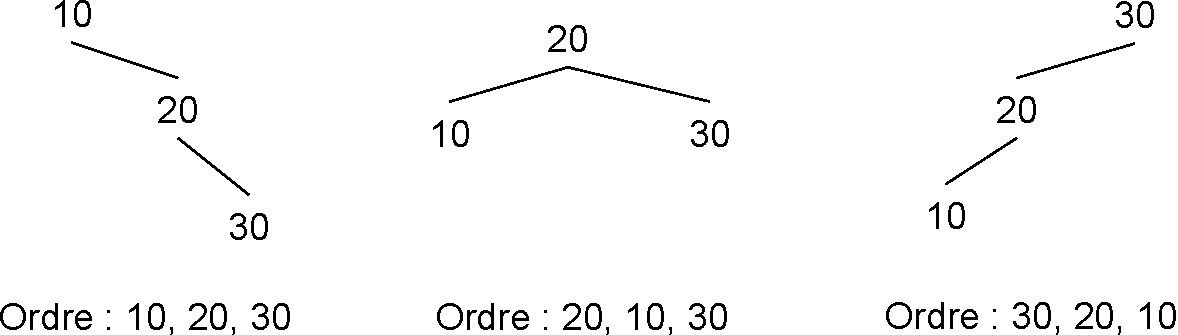
\includegraphics[scale=0.5]{figs/tree_insert}
\end{figure}
\end{frame}

\begin{frame}{Suppression}{Cas 1}
Le n\oe ud à supprimer est une feuille.
\begin{figure}
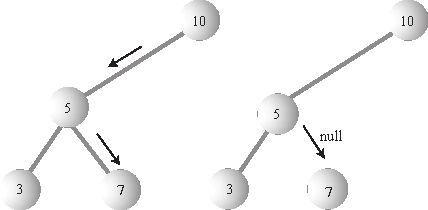
\includegraphics[scale=1]{figs/del1_tree}
\end{figure}
\hspace{3em}a)Avant suppression  \hspace{1em}  b)Après suppression de 7
\end{frame}
\begin{frame}[fragile]{Suppression}{Cas 1 : Version itérative}
\begin{lstlisting}[language=Java]
public boolean suppression(int cle){
  Noeud courant = racine;
  Noeud parent = racine;
  boolean estFilsGauche = true;
  while(courant.cle != cle){
   parent = courant;
     if(cle < courant.cle){
      estFilsGauche = true;
      courant = courant.filsGauche;
   }else{
     estFilsGauche = false;
     courant = courant.filsDroit;
   }
   if(courant == null)
     return false;
  } // fin while, courant pointe le noeud a effacer
\end{lstlisting}
\end{frame}


\begin{frame}[fragile]{Suppression}{Cas 1 : Version itérative}
\begin{lstlisting}[language=Java]
// suite de la suppression cas 1
  if(courant.filsGauche==null &&
   courant.filsDroit==null){
    if(courant == racine)
     racine = null;
    else if(estFilsGauche)
     parent.filsGauche = null;
    else
     parent.filsDroit = null;
}
\end{lstlisting}
\end{frame}

\begin{frame}{Suppression}{Cas 2}
Le n\oe ud à supprimer a un unique fils.
\begin{figure}
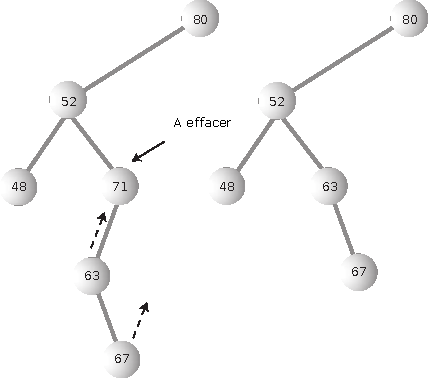
\includegraphics[scale=0.8]{figs/del2_tree}
\end{figure}
\hspace{3em}a)Avant suppression  \hspace{1em}  b)Après suppression de 71
\end{frame}

\begin{frame}[fragile]{Suppression}{Cas 2 : Version itérative}
\begin{lstlisting}[language=Java]
//Suite de traitement du 1er cas
//pas de fils droit on remplace avec le ss-arbre G
else if(courant.filsDroit==null)
  if(courant == racine)
   racine = courant.filsGauche;
  else if(estFilsGauche)
   parent.filsGauche = courant.filsGauche;
  else parent.filsDroit = courant.filsGauche;
//pas de fils gauche on remplace avec le ss-arbre D
else if(courant.filsGauche==null)
  if(courant == racine)
   racine = courant.filsDroit;
  else if(estFilsGauche)
   parent.filsGauche = courant.filsDroit;
  else parent.filsDroit = courant.filsDroit;
\end{lstlisting}
\end{frame}



\begin{frame}{Suppression}{Cas 3}
Le n\oe ud à supprimer a deux fils.
\begin{figure}
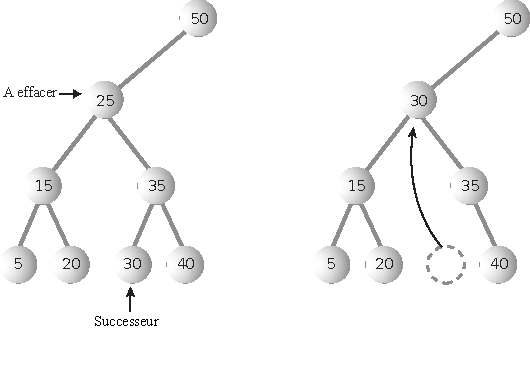
\includegraphics[scale=0.8]{figs/del3_tree}
\end{figure}
\hspace{3em}a)Avant suppression \hspace{1em}  b)Après suppression de 25
\end{frame}

\begin{frame}{Suppression}{Cas 3}
Recherche du successeur :
\begin{itemize}
\item On a besoin d'identifier le \hl{successeur} du n\oe ud à supprimer
\item Si le n\oe ud à supprimer a un fils droit
\begin{itemize}
\item Il s'agit du n\oe ud avec la clé minimum des successeurs
\item Il s'agit donc du n\oe ud de clé minimum du sous-arbre droit du n\oe ud à supprimer
\end{itemize}
\item Sinon c'est le premier père droit en remontant la branche du n\oe ud à supprimer.
\item Respectivement, le \hl{prédécesseur} : n\oe ud de clé maximum dans le sous-arbre gauche du  n\oe ud à supprimer sinon le premier père gauche si pas de fils droit
\end{itemize}
\end{frame}

\begin{frame}[fragile]{Suppression}{Recherche du successeur(si fils doit non null)}

\begin{lstlisting}[language=Java]
public Noeud successeur(Noeud noeud){
  return minimum(noeud.filsDroit);
}

public Noeud predecesseur(Noeud noeud){
  return maximum(noeud.filsGauche);
}
\end{lstlisting}
Si on veut mettre le successeur à la place d'un n\oe ud à supprimer:
\begin{itemize}
\item il faut "détacher" le successeur
\item et mettre à jour les références
\end{itemize} 
\end{frame}

\begin{frame}[fragile]{Suppression}{Recherche du successeur(si fils doit non null)}
\begin{lstlisting}[language=Java]
Noeud getSuccesseur(Noeud supNoeud){
  Noeud parentSuccesseur = supNoeud;
  Noeud successeur = supNoeud;
  Noeud courant = supNoeud.filsDroit;
   while(courant != null){
    parentSuccesseur = successeur;
    successeur = courant;
    courant = courant.filsGauche;
   }
   //Si succ. = fils droit de supNoeud rien a faire
   if(successeur != supNoeud.filsDroit){
    //MAJ des references
    parentSuccesseur.filsGauche = successeur.filsDroit;
    successeur.filsDroit = supNoeud.filsDroit;
   }
 return successeur;
}
\end{lstlisting}
\end{frame}

\begin{frame}[fragile]{Suppression}{Cas 3 : Version itérative}
\begin{lstlisting}[language=Java]
//Suite de traitement du 1er et 2eme cas
// deux fils, on remplace par le successeur
else {
  //on recupere le successeur du noeud courant
  //mais on doit aussi le detacher
  Noeud successeur = getSuccesseur(courant);
  //connecte le pere du noeud courant au successeur
  if(courant == racine)
   racine = successeur;
  else if(estFilsGauche)
   parent.filsGauche = successeur;
  else parent.filsDroit = successeur;
  //connecte le successeur au fils gauche du courant
  successeur.filsGauche = courant.filsGauche;
 }return true; //Fin de la suppression du cas 3
}//(un successeur ne peut pas avoir de fils gauche)
\end{lstlisting}
\end{frame}

\begin{frame}{Implémentation Java}
\begin{itemize}
\item Pas d'implémentation directement manipulable d'ABR en Java
\item Mais utilisés pour l'implémentation de Map (\hl{TreeMap}) ou de Set (\hl{TreeSet}) (à l'instar des tables de hachages).
\end{itemize}
\end{frame}



\end{document}

